\documentclass[11pt,]{article}
\usepackage[left=1in,top=1in,right=1in,bottom=1in]{geometry}
\newcommand*{\authorfont}{\fontfamily{phv}\selectfont}
\usepackage[]{mathpazo}


  \usepackage[T1]{fontenc}
  \usepackage[utf8]{inputenc}



\usepackage{abstract}
\renewcommand{\abstractname}{}    % clear the title
\renewcommand{\absnamepos}{empty} % originally center

\renewenvironment{abstract}
 {{%
    \setlength{\leftmargin}{0mm}
    \setlength{\rightmargin}{\leftmargin}%
  }%
  \relax}
 {\endlist}

\makeatletter
\def\@maketitle{%
  \newpage
%  \null
%  \vskip 2em%
%  \begin{center}%
  \let \footnote \thanks
    {\fontsize{18}{20}\selectfont\raggedright  \setlength{\parindent}{0pt} \@title \par}%
}
%\fi
\makeatother




\setcounter{secnumdepth}{0}

\usepackage{color}
\usepackage{fancyvrb}
\newcommand{\VerbBar}{|}
\newcommand{\VERB}{\Verb[commandchars=\\\{\}]}
\DefineVerbatimEnvironment{Highlighting}{Verbatim}{commandchars=\\\{\}}
% Add ',fontsize=\small' for more characters per line
\usepackage{framed}
\definecolor{shadecolor}{RGB}{248,248,248}
\newenvironment{Shaded}{\begin{snugshade}}{\end{snugshade}}
\newcommand{\KeywordTok}[1]{\textcolor[rgb]{0.13,0.29,0.53}{\textbf{{#1}}}}
\newcommand{\DataTypeTok}[1]{\textcolor[rgb]{0.13,0.29,0.53}{{#1}}}
\newcommand{\DecValTok}[1]{\textcolor[rgb]{0.00,0.00,0.81}{{#1}}}
\newcommand{\BaseNTok}[1]{\textcolor[rgb]{0.00,0.00,0.81}{{#1}}}
\newcommand{\FloatTok}[1]{\textcolor[rgb]{0.00,0.00,0.81}{{#1}}}
\newcommand{\ConstantTok}[1]{\textcolor[rgb]{0.00,0.00,0.00}{{#1}}}
\newcommand{\CharTok}[1]{\textcolor[rgb]{0.31,0.60,0.02}{{#1}}}
\newcommand{\SpecialCharTok}[1]{\textcolor[rgb]{0.00,0.00,0.00}{{#1}}}
\newcommand{\StringTok}[1]{\textcolor[rgb]{0.31,0.60,0.02}{{#1}}}
\newcommand{\VerbatimStringTok}[1]{\textcolor[rgb]{0.31,0.60,0.02}{{#1}}}
\newcommand{\SpecialStringTok}[1]{\textcolor[rgb]{0.31,0.60,0.02}{{#1}}}
\newcommand{\ImportTok}[1]{{#1}}
\newcommand{\CommentTok}[1]{\textcolor[rgb]{0.56,0.35,0.01}{\textit{{#1}}}}
\newcommand{\DocumentationTok}[1]{\textcolor[rgb]{0.56,0.35,0.01}{\textbf{\textit{{#1}}}}}
\newcommand{\AnnotationTok}[1]{\textcolor[rgb]{0.56,0.35,0.01}{\textbf{\textit{{#1}}}}}
\newcommand{\CommentVarTok}[1]{\textcolor[rgb]{0.56,0.35,0.01}{\textbf{\textit{{#1}}}}}
\newcommand{\OtherTok}[1]{\textcolor[rgb]{0.56,0.35,0.01}{{#1}}}
\newcommand{\FunctionTok}[1]{\textcolor[rgb]{0.00,0.00,0.00}{{#1}}}
\newcommand{\VariableTok}[1]{\textcolor[rgb]{0.00,0.00,0.00}{{#1}}}
\newcommand{\ControlFlowTok}[1]{\textcolor[rgb]{0.13,0.29,0.53}{\textbf{{#1}}}}
\newcommand{\OperatorTok}[1]{\textcolor[rgb]{0.81,0.36,0.00}{\textbf{{#1}}}}
\newcommand{\BuiltInTok}[1]{{#1}}
\newcommand{\ExtensionTok}[1]{{#1}}
\newcommand{\PreprocessorTok}[1]{\textcolor[rgb]{0.56,0.35,0.01}{\textit{{#1}}}}
\newcommand{\AttributeTok}[1]{\textcolor[rgb]{0.77,0.63,0.00}{{#1}}}
\newcommand{\RegionMarkerTok}[1]{{#1}}
\newcommand{\InformationTok}[1]{\textcolor[rgb]{0.56,0.35,0.01}{\textbf{\textit{{#1}}}}}
\newcommand{\WarningTok}[1]{\textcolor[rgb]{0.56,0.35,0.01}{\textbf{\textit{{#1}}}}}
\newcommand{\AlertTok}[1]{\textcolor[rgb]{0.94,0.16,0.16}{{#1}}}
\newcommand{\ErrorTok}[1]{\textcolor[rgb]{0.64,0.00,0.00}{\textbf{{#1}}}}
\newcommand{\NormalTok}[1]{{#1}}

\usepackage{graphicx}
% We will generate all images so they have a width \maxwidth. This means
% that they will get their normal width if they fit onto the page, but
% are scaled down if they would overflow the margins.
\makeatletter
\def\maxwidth{\ifdim\Gin@nat@width>\linewidth\linewidth
\else\Gin@nat@width\fi}
\makeatother
\let\Oldincludegraphics\includegraphics
\renewcommand{\includegraphics}[1]{\Oldincludegraphics[width=\maxwidth]{#1}}

\title{A Pandoc Markdown Article Starter and Template \thanks{Replication files are available on the author's Github account
(\url{http://github.com/svmiller}). \textbf{Current version}: December
17, 2016; \textbf{Corresponding author}:
\href{mailto:svmille@clemson.edu}{\nolinkurl{svmille@clemson.edu}}.}  }



\author{\Large Steven V. Miller\vspace{0.05in} \newline\normalsize\emph{Clemson University}  }


\date{}

\usepackage{titlesec}

\titleformat*{\section}{\normalsize\bfseries}
\titleformat*{\subsection}{\normalsize\itshape}
\titleformat*{\subsubsection}{\normalsize\itshape}
\titleformat*{\paragraph}{\normalsize\itshape}
\titleformat*{\subparagraph}{\normalsize\itshape}


\usepackage{natbib}
\bibliographystyle{apsr}



\newtheorem{hypothesis}{Hypothesis}
\usepackage{setspace}

\makeatletter
\@ifpackageloaded{hyperref}{}{%
\ifxetex
  \usepackage[setpagesize=false, % page size defined by xetex
              unicode=false, % unicode breaks when used with xetex
              xetex]{hyperref}
\else
  \usepackage[unicode=true]{hyperref}
\fi
}
\@ifpackageloaded{color}{
    \PassOptionsToPackage{usenames,dvipsnames}{color}
}{%
    \usepackage[usenames,dvipsnames]{color}
}
\makeatother
\hypersetup{breaklinks=true,
            bookmarks=true,
            pdfauthor={Steven V. Miller (Clemson University)},
             pdfkeywords = {pandoc, r markdown, knitr},  
            pdftitle={A Pandoc Markdown Article Starter and Template},
            colorlinks=true,
            citecolor=blue,
            urlcolor=blue,
            linkcolor=magenta,
            pdfborder={0 0 0}}
\urlstyle{same}  % don't use monospace font for urls



\begin{document}
	
% \pagenumbering{arabic}% resets `page` counter to 1 
%
% \maketitle

{% \usefont{T1}{pnc}{m}{n}
\setlength{\parindent}{0pt}
\thispagestyle{plain}
{\fontsize{18}{20}\selectfont\raggedright 
\maketitle  % title \par  

}

{
   \vskip 13.5pt\relax \normalsize\fontsize{11}{12} 
\textbf{\authorfont Steven V. Miller} \hskip 15pt \emph{\small Clemson University}   

}

}







\begin{abstract}

    \hbox{\vrule height .2pt width 39.14pc}

    \vskip 8.5pt % \small 

\noindent This document provides an introduction to R Markdown, argues for its
benefits, and presents a sample manuscript template intended for an
academic audience. I include basic syntax to R Markdown and a minimal
working example of how the analysis itself can be conducted within R
with the \texttt{knitr} package.


\vskip 8.5pt \noindent \emph{Keywords}: pandoc, r markdown, knitr \par

    \hbox{\vrule height .2pt width 39.14pc}



\end{abstract}


\vskip 6.5pt

\noindent  \section{Introduction}\label{introduction}

Academic workflow, certainly in political science, is at a crossroads.
The \emph{American Journal of Political Science} (\emph{AJPS}) announced
a (my words)
\href{http://ajps.org/2015/03/26/the-ajps-replication-policy-innovations-and-revisions/}{``show
your work'' initiative} in which authors who are tentatively accepted
for publication at the journal must hand over the raw code and data that
produced the results shown in the manuscript. The editorial team at
\emph{AJPS} then reproduces the code from the manuscript. Pending
successful replication, the manuscript moves toward publication. The
\emph{AJPS} might be at the fore of this movement, and it could be the
most aggressive among political science journals, but other journals in
our field have signed the joint
\href{http://www.dartstatement.org/}{Data Access \& Research
Transparency} (DART) initiative. This, at a bare minimum, requires
uploading code from quantitatively-oriented published articles to
in-house directories hosted by the journal or to services like
\href{http://dataverse.org/}{Dataverse}.

There are workflow implications to the Lacour controversy as well.
Political science, for the foreseeable future, will struggle with the
extent of
\href{http://stanford.edu/~dbroock/broockman_kalla_aronow_lg_irregularities.pdf}{the
data fraud perpetrated by Michael Lacour} in an article co-authored with
Donald P. Green in \emph{Science}, the general scientific journal of
record in the United States. A failure to reproduce LaCour's results
with different samples uncovered a comprehensive effort by LaCour to
``fake'' data that provided results to what we felt or believed to be
true \href{http://chronicle.com/article/LAffaire-LaCour/230905/}{(i.e.
``truthiness'')}. However,
\href{http://kieranhealy.org/blog/archives/2015/05/20/fake-science-real-consequences/}{fake
data can have real consequences} for both the researcher and those who
want to learn from it and use it for various purposes. Even research
done honestly may suffer the same fate if researchers are not diligent
in their workflow.

These recent events underscore the DART push and cast a shadow over our
workflow. However, good workflow has always been an issue in our
discipline. Cloud storage services like
\href{http://www.dropbox.com}{Dropbox} are still relatively new among
political scientists. Without cloud storage, previous workflow left open
the possibility that work between a home computer and an office computer
was lost as a function of a corrupted thumb drive, an overheated power
supply, or, among other things, the wave of viruses that
\href{http://money.cnn.com/2003/11/05/technology/microsoftbounty/}{would
particularly affect Microsoft users every summer}. Social sciences,
\href{http://kieranhealy.org/blog/archives/2014/01/23/plain-text/}{unlike
engineering}, have traditionally relied on software like Microsoft Word
for manuscript preparation though any word processor reduces workflow to
a series of clicks and strokes on a keyboard. This is
\href{http://www.nytimes.com/2013/04/19/opinion/krugman-the-excel-depression.html}{a
terrible way to track changes} or maintain version control. The addition
of collaborators only compounds all the aforementioned issues. The
proverbial left hand may not know what the right hand is doing.

I think there is reason for optimism. We only struggle with it now
because we have tools like \href{http://rmarkdown.rstudio.com/}{R
Markdown} and \href{http://pandoc.org/}{Pandoc}, more generally, that
make significant strides in workflow. LaTeX resolved earlier issues of
corrupted binary files by reducing documents to raw markup that was
little more than raw text and revisions that could be easily kept as
\href{http://tex.stackexchange.com/questions/11177/how-to-write-hidden-notes-in-a-latex-file}{``commented''
text}. However, for all its benefits (including pretty PDFs),
\href{http://www-rohan.sdsu.edu/~aty/bibliog/latex/gripe.html}{LaTeX is
\emph{ugly} code} and does not provide means of seamlessly working with
the actual data analysis itself. R Markdown both eliminates markup and
allows the author and her collaborators to write and reproduce the
manuscript in one fell swoop.

\section{Getting Started with YAML}\label{getting-started-with-yaml}

The lion's share of a R Markdown document will be raw text, though the
front matter may be the most important part of the document. R Markdown
uses \href{http://www.yaml.org/}{YAML} for its metadata and the fields
differ from
\href{http://svmiller.com/blog/2015/02/moving-from-beamer-to-r-markdown/}{what
an author would use for a Beamer presentation}. I provide a sample YAML
metadata largely taken from this exact document and explain it below.

\begin{Shaded}
\begin{Highlighting}[]
\NormalTok{---}
\NormalTok{output:}\StringTok{ }
\StringTok{  }\NormalTok{pdf_document:}
\StringTok{    }\NormalTok{citation_package:}\StringTok{ }\NormalTok{natbib}
    \NormalTok{keep_tex:}\StringTok{ }\NormalTok{true}
    \NormalTok{fig_caption:}\StringTok{ }\NormalTok{true}
    \NormalTok{latex_engine:}\StringTok{ }\NormalTok{pdflatex}
    \NormalTok{template:}\StringTok{ }\ErrorTok{~/}\NormalTok{Dropbox/miscelanea/svm-r-markdown-templates/svm.latex.ms.tex}
\NormalTok{title:}\StringTok{ "A Pandoc Markdown Article Starter and Template"}
\NormalTok{thanks:}\StringTok{ "Replication files are available on the author's Github account..."}
\NormalTok{author:}
\NormalTok{-}\StringTok{ }\NormalTok{name:}\StringTok{ }\NormalTok{Steven V. Miller}
  \NormalTok{affiliation:}\StringTok{ }\NormalTok{Clemson University}
\NormalTok{-}\StringTok{ }\NormalTok{name:}\StringTok{ }\NormalTok{Mary Margaret Albright}
  \NormalTok{affiliation:}\StringTok{ }\NormalTok{Pendelton State University}
\NormalTok{-}\StringTok{ }\NormalTok{name:}\StringTok{ }\NormalTok{Rembrandt Q. Einstein}
  \NormalTok{affiliation:}\StringTok{ }\NormalTok{Springfield University}
\NormalTok{abstract:}\StringTok{ "This document provides an introduction to R Markdown, argues for its..."}
\NormalTok{keywords:}\StringTok{ "pandoc, r markdown, knitr"}
\NormalTok{date:}\StringTok{ "`r format(Sys.time(), '%B %d, %Y')`"}
\NormalTok{geometry:}\StringTok{ }\NormalTok{margin=1in}
\NormalTok{fontfamily:}\StringTok{ }\NormalTok{mathpazo}
\NormalTok{fontsize:}\StringTok{ }\NormalTok{11pt}
\CommentTok{# spacing: double}
\NormalTok{bibliography:}\StringTok{ }\ErrorTok{~/}\NormalTok{Dropbox/master.bib}
\NormalTok{biblio-style:}\StringTok{ }\NormalTok{apsr}
\NormalTok{---}
\end{Highlighting}
\end{Shaded}

\texttt{output:} will tell R Markdown we want a PDF document rendered
with LaTeX. Since we are adding a fair bit of custom options to this
call, we specify \texttt{pdf\_document:} on the next line (with,
importantly, a two-space indent). We specify additional output-level
options underneath it, each are indented with four spaces.
\texttt{citation\_package:\ natbib} tells R Markdown to use
\texttt{natbib} to handle bibliographic citations.\footnote{R Markdown
  can use Pandoc's native bibliography management system or even
  \texttt{biblatex}, but I've found that it chokes with some of the more
  advanced stuff I've done with my .bib file over the years. For
  example, I've been diligent about special characters (e.g.~umlauts and
  acute accents) in author names in my .bib file, but Pandoc's native
  citation system will choke on these characters in a .bib file. I
  effectively need \texttt{natbib} for my own projects.} Thereafter, the
next line (\texttt{keep\_tex:\ true}) tells R Markdown to render a raw
\texttt{.tex} file along with the PDF document. This is useful for both
debugging and the publication stage, when the editorial team will ask
for the raw \texttt{.tex} so that they could render it and later provide
page proofs. The next line \texttt{fig\_caption:\ true} tells R Markdown
to make sure that whatever images are included in the document are
treated as figures in which our caption in brackets in a Markdown call
is treated as the caption in the figure. The next line
(\texttt{latex\_engine:\ pdflatex}) tells R Markdown to use pdflatex and
not some other option like \texttt{lualatex}. For my template, I'm
pretty sure this is mandatory.\footnote{The main reason I still use
  \texttt{pdflatex} (and most readers probably do as well) is because of
  LaTeX fonts.
  \href{http://www-rohan.sdsu.edu/~aty/bibliog/latex/gripe.html}{Unlike
  others}, I find standard LaTeX fonts to be appealing.}

The next line (\texttt{template:\ ...}) tells R Markdown to use my
custom LaTeX template.\footnote{Notice that the path is relative. The
  user can, if she wishes, install this in the default Pandoc directory.
  I don't think this is necessary. Just be mindful of wherever the
  template is placed. Importantly, \texttt{\textasciitilde{}} is used in
  R to find the home directory (not necessarily the working directory).
  It is equivalent to saying \texttt{/home/steve} in Linux, or
  \texttt{/Users/steve} on a Mac, in my case.} While I will own any
errors in the code, I confess to ``Frankensteining'' this template from
\href{https://github.com/jgm/pandoc-templates}{the default LaTeX
template} from Pandoc,
\href{https://github.com/kjhealy/pandoc-templates/tree/master/templates}{Kieran
Healy's LaTeX template}, and liberally using raw TeX from the
\href{https://www.acm.org/publications/article-templates/acm-latex-style-guide}{Association
for Computing Machinery's (ACM) LaTeX template}. I rather like that
template since it resembles standard manuscripts when they are published
in some of our more prominent journals. I will continue with a
description of the YAML metadata in the next paragraph, though invite
the curious reader to scroll to the end of the accompanying post to see
the PDF this template produces.

The next fields get to the heart of the document itself. \texttt{title:}
is, intuitively, the title of the manuscript. Do note that fields like
\texttt{title:} do not have to be in quotation marks, but must be in
quotation marks if the title of the document includes a colon. That
said, the only reason to use a colon in an article title is if it is
followed by a subtitle, hence the optional field (\texttt{subtitle:}).
Notice I ``comment out'' the subtitle in the above example with a pound
sign since this particular document does not have a subtitle. If
\texttt{thanks:} is included and has an accompanying entry, the ensuing
title of the document gets an asterisk and a footnote. This field is
typically used to advise readers that the document is a working paper or
is forthcoming in a journal.

The next field (\texttt{author:}) is a divergence from standard YAML,
but I think it is useful. I will also confess to pilfering this idea
from Kieran Healy's template. Typically, multiple authors for a given
document are separated by an \texttt{\textbackslash{}and} in this field.
However, standard LaTeX then creates a tabular field separating multiple
authors that is somewhat restrictive and not easy to override. As a
result, I use this setup (again, taken from Kieran Healy) to sidestep
the restrictive rendering of authors in the standard
\texttt{\textbackslash{}maketitle} tag. After \texttt{author:}, enter
\texttt{-\ name:} (no space before the dash) and fill in the field with
the first author. On the next line, enter two spaces, followed by
\texttt{affiliation:} and the institute or university affiliation of the
first author.

Do notice this can be repeated for however many co-authors there are to
a manuscript. The rendered PDF will enter each co-author in a new line
in a manner similar to journals like \emph{American Journal of Political
Science}, \emph{American Political Science Review}, or \emph{Journal of
Politics}.

The next two fields pertain to the frontmatter of a manuscript. They
should also be intuitive for the reader. \texttt{abstract} should
contain the abstract and \texttt{keywords} should contain some keywords
that describe the research project. Both fields are optional, though are
practically mandatory. Every manuscript requires an abstract and some
journals---especially those published by Sage---request them with
submitted manuscripts. My template also includes these keywords in the
PDF's metadata.

\texttt{date} comes standard with R Markdown and you can use it to enter
the date of the most recent compile. I typically include the date of the
last compile for a working paper in the \texttt{thanks:} field, so this
field currently does not do anything in my Markdown-LaTeX manuscript
template. I include it in my YAML as a legacy, basically.

The next items are optional and cosmetic. \texttt{geometry:} is a
standard option in LaTeX. I set the margins at one inch, and you
probably should too. \texttt{fontfamily:} is optional, but I use it to
specify the Palatino font. The default option is Computer Modern Roman.
\texttt{fontsize:} sets, intuitively, the font size. The default is
10-point, but I prefer 11-point. \texttt{spacing:} is an optional field.
If it is set as ``double'', the ensuing document is double-spaced.
``single'' is the only other valid entry for this field, though not
including the entry in the YAML metadata amounts to singlespacing the
document by default. Notice I have this ``commented out'' in the example
code.

The final two options pertain to the bibliography.
\texttt{bibliography:} specifies the location of the .bib file, so the
author could make citations in the manuscript. \texttt{biblio-style}
specifies the type of bibliography to use. You'll typically set this as
APSR. You could also specify the relative path of
\href{http://svmiller.com/miscellany/journal-of-peace-research-bst-file/}{my
\emph{Journal of Peace Research} .bst file} if you are submitting to
that journal.

\section{Getting Started with Markdown
Syntax}\label{getting-started-with-markdown-syntax}

There are a lot of cheatsheets and reference guides for Markdown (e.g.
\href{https://github.com/adam-p/markdown-here/wiki/Markdown-Cheatsheet}{Adam
Prichard},
\href{http://assemble.io/docs/Cheatsheet-Markdown.html}{Assemble},
\href{https://www.rstudio.com/wp-content/uploads/2015/02/rmarkdown-cheatsheet.pdf}{Rstudio},
\href{https://www.rstudio.com/wp-content/uploads/2015/03/rmarkdown-reference.pdf}{Rstudio
again},
\href{http://scottboms.com/downloads/documentation/markdown_cheatsheet.pdf}{Scott
Boms}, \href{https://daringfireball.net/projects/markdown/syntax}{Daring
Fireball}, among, I'm sure, several others). I encourage the reader to
look at those, though I will retread these references here with a
minimal working example below.

\begin{Shaded}
\begin{Highlighting}[]

\FunctionTok{# Introduction}

\NormalTok{**Lorem ipsum** dolor *sit amet*. }

\NormalTok{- }\FloatTok{Single asterisks italicize text *like this*. }
\FloatTok{- Double asterisks embolden text **like this**.}

\FloatTok{Start a new paragraph with a blank line separating paragraphs.}

\FloatTok{- This will start an unordered list environment, and this will be the first item.}
\FloatTok{- This will be a second item.}
\FloatTok{- A third item.}
\FloatTok{    - Four spaces and a dash create a sublist and this item in it.}
\FloatTok{- The fourth item.}
\FloatTok{  }  
\FloatTok{1. This starts a numerical list.}
\FloatTok{2. This is no. 2 in the numerical list.}
\FloatTok{  }  
\FloatTok{# This Starts A New Section}
\FloatTok{## This is a Subsection}
\FloatTok{### This is a Subsubsection}
\FloatTok{#### This starts a Paragraph Block.}

\FloatTok{> This will create a block quote, if you want one.}

\FloatTok{Want a table? This will create one.}

\FloatTok{Table Header  | Second Header}
\FloatTok{------------- | -------------}
\FloatTok{Table Cell    | Cell 2}
\FloatTok{Cell 3        | Cell 4 }

\FloatTok{Note that the separators *do not* have to be aligned.}

\FloatTok{Want an image? This will do it.}

\AlertTok{![caption for my image](path/to/image.jpg)}

\BaseNTok{`fig_caption: yes`}\FloatTok{ will provide a caption. Put that in the YAML metadata.}

\FloatTok{Almost forgot about creating a footnote.}\OtherTok{[^1]}\FloatTok{ This will do it again.}\OtherTok{[^2]}

\OtherTok{[^1]}\FloatTok{: The first footnote}
\OtherTok{[^2]}\FloatTok{: The second footnote}

\FloatTok{Want to cite something? }

\FloatTok{- Find your biblatexkey in your bib file.}
\FloatTok{- Put an @ before it, like @smith1984, or whatever it is.}
\FloatTok{- @smith1984 creates an in-text citation (e.g. Smith (1984) says...)}
\FloatTok{- [@smith1984] creates a parenthetical citation (Smith, 1984)}

\FloatTok{That'll also automatically create a reference list at the end of the document.}

\OtherTok{[In-text link to Google](http://google.com)}\FloatTok{ as well.}
\end{Highlighting}
\end{Shaded}

That's honestly it. Markdown takes the chore of markup from your
manuscript (hence: ``Markdown'').

On that note, you could easily pass most LaTeX code through Markdown if
you're writing a LaTeX document. However, you don't need to do this
(unless you're using the math environment) and probably shouldn't anyway
if you intend to share your document in HTML as well.

\section{Using R Markdown with Knitr}\label{using-r-markdown-with-knitr}

Perhaps the greatest intrigue of R Markdown comes with the
\href{http://yihui.name/knitr/}{\texttt{knitr} package} provided by
\citet{xie2013ddrk}. In other words, the author can, if she chooses, do
the analysis in the Markdown document itself and compile/execute it in
R.

Take, for example, this simple exercise using the \texttt{voteincome}
data from the \texttt{Zelig} package. Suppose I want to explain the
decision to vote using data from this package. I load in the data, clean
the data, run the analyses, and present the results as a coefficient
plot.

Here's what this code looks like. All I did was create a code display,
which starts with three \emph{backticks} (i.e.~those ticks next to the
number 1 key on your keyboard) and ends with three backticks on another
line. On the first line of backticks (i.e.~to start the code display)
enter \texttt{\{r,\ eval=FALSE,\ tidy=TRUE\}}. The \texttt{eval=FALSE}
option just displays the R code (and does not run it),
\texttt{tidy=TRUE} wraps long code so it does not run off the page.

Within that code display, I enter my R code like this.

\begin{Shaded}
\begin{Highlighting}[]
\KeywordTok{suppressMessages}\NormalTok{(}\KeywordTok{library}\NormalTok{(Zelig))}
\KeywordTok{suppressMessages}\NormalTok{(}\KeywordTok{library}\NormalTok{(arm))}
\KeywordTok{suppressMessages}\NormalTok{(}\KeywordTok{library}\NormalTok{(coefplot))}

\KeywordTok{data}\NormalTok{(voteincome)}

\NormalTok{voteincome$z.age <-}\StringTok{ }\NormalTok{arm::}\KeywordTok{rescale}\NormalTok{(voteincome$age)}
\NormalTok{voteincome$z.education <-}\StringTok{ }\NormalTok{arm::}\KeywordTok{rescale}\NormalTok{(voteincome$education)}
\NormalTok{voteincome$z.income <-}\StringTok{ }\NormalTok{arm::}\KeywordTok{rescale}\NormalTok{(voteincome$income)}

\NormalTok{M1 <-}\StringTok{ }\KeywordTok{glm}\NormalTok{(vote ~}\StringTok{ }\NormalTok{z.age +}\StringTok{ }\NormalTok{female +}\StringTok{ }\NormalTok{z.education +}\StringTok{ }\NormalTok{z.income, }\DataTypeTok{data =} \NormalTok{voteincome, }
    \DataTypeTok{family =} \NormalTok{binomial)}

\KeywordTok{coefplot}\NormalTok{(M1)}
\end{Highlighting}
\end{Shaded}

The implications for workflow are faily substantial. Authors can rather
quickly display the code they used to run the analyses in the document
itself (likely in the appendix). As such, there's little guesswork for
reviewers and editors in understanding what the author did in the
analyses reported in the manuscript.

It doesn't end there. In fact, here's what happens when
\texttt{eval=FALSE} is omitted or changed to \texttt{eval=TRUE}. Now,
the code runs within R. Observe.

\begin{Shaded}
\begin{Highlighting}[]
\KeywordTok{suppressMessages}\NormalTok{(}\KeywordTok{library}\NormalTok{(Zelig))}
\KeywordTok{suppressMessages}\NormalTok{(}\KeywordTok{library}\NormalTok{(arm))}


\KeywordTok{data}\NormalTok{(voteincome)}

\NormalTok{voteincome$z.age <-}\StringTok{ }\NormalTok{arm::}\KeywordTok{rescale}\NormalTok{(voteincome$age)}
\NormalTok{voteincome$z.education <-}\StringTok{ }\NormalTok{arm::}\KeywordTok{rescale}\NormalTok{(voteincome$education)}
\NormalTok{voteincome$z.income <-}\StringTok{ }\NormalTok{arm::}\KeywordTok{rescale}\NormalTok{(voteincome$income)}

\NormalTok{M1 <-}\StringTok{ }\KeywordTok{glm}\NormalTok{(vote ~}\StringTok{ }\NormalTok{z.age +}\StringTok{ }\NormalTok{female +}\StringTok{ }\NormalTok{z.education +}\StringTok{ }\NormalTok{z.income, }\DataTypeTok{data =} \NormalTok{voteincome, }
    \DataTypeTok{family =} \NormalTok{binomial)}

\NormalTok{arm::}\KeywordTok{coefplot}\NormalTok{(M1)}
\end{Highlighting}
\end{Shaded}

\begin{figure}
\centering
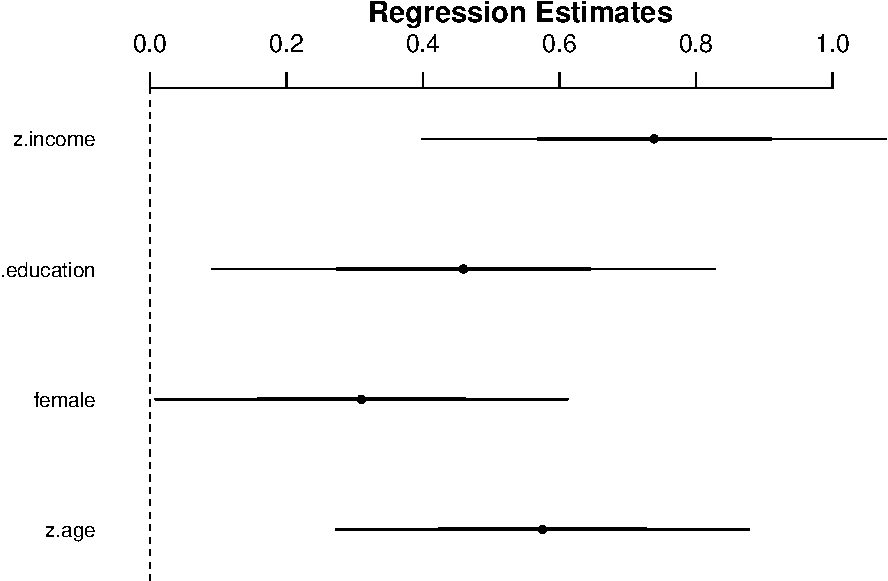
\includegraphics{svm-rmarkdown-article-example_files/figure-latex/unnamed-chunk-3-1.pdf}
\caption{A Coefficient Plot}
\end{figure}

To get \texttt{knitr} to present the results of a table, add
\texttt{results="asis"} to the brackets to start the R code chunk. The
ensuing output will look like this (though the table may come on the
next page).

\begin{Shaded}
\begin{Highlighting}[]
\KeywordTok{suppressMessages}\NormalTok{(}\KeywordTok{library}\NormalTok{(Zelig))}
\KeywordTok{suppressMessages}\NormalTok{(}\KeywordTok{library}\NormalTok{(stargazer))}
\KeywordTok{suppressMessages}\NormalTok{(}\KeywordTok{library}\NormalTok{(arm))}

\KeywordTok{data}\NormalTok{(voteincome)}

\NormalTok{voteincome$z.age <-}\StringTok{ }\NormalTok{arm::}\KeywordTok{rescale}\NormalTok{(voteincome$age)}
\NormalTok{voteincome$z.education <-}\StringTok{ }\NormalTok{arm::}\KeywordTok{rescale}\NormalTok{(voteincome$education)}
\NormalTok{voteincome$z.income <-}\StringTok{ }\NormalTok{arm::}\KeywordTok{rescale}\NormalTok{(voteincome$income)}


\NormalTok{M1 <-}\StringTok{ }\KeywordTok{glm}\NormalTok{(vote ~}\StringTok{ }\NormalTok{z.age +}\StringTok{ }\NormalTok{female +}\StringTok{ }\NormalTok{z.education +}\StringTok{ }\NormalTok{z.income, }\DataTypeTok{data =} \NormalTok{voteincome, }
    \DataTypeTok{family =} \NormalTok{binomial)}

\KeywordTok{stargazer}\NormalTok{(M1, }\DataTypeTok{title =} \StringTok{"A Handsome Table"}\NormalTok{, }\DataTypeTok{header =} \OtherTok{FALSE}\NormalTok{)}
\end{Highlighting}
\end{Shaded}

\begin{table}[!htbp] \centering 
  \caption{A Handsome Table} 
  \label{} 
\begin{tabular}{@{\extracolsep{5pt}}lc} 
\\[-1.8ex]\hline 
\hline \\[-1.8ex] 
 & \multicolumn{1}{c}{\textit{Dependent variable:}} \\ 
\cline{2-2} 
\\[-1.8ex] & vote \\ 
\hline \\[-1.8ex] 
 z.age & 0.575$^{***}$ \\ 
  & (0.151) \\ 
  & \\ 
 female & 0.310$^{**}$ \\ 
  & (0.151) \\ 
  & \\ 
 z.education & 0.459$^{**}$ \\ 
  & (0.184) \\ 
  & \\ 
 z.income & 0.739$^{***}$ \\ 
  & (0.170) \\ 
  & \\ 
 Constant & 1.706$^{***}$ \\ 
  & (0.110) \\ 
  & \\ 
\hline \\[-1.8ex] 
Observations & 1,500 \\ 
Log Likelihood & $-$592.801 \\ 
Akaike Inf. Crit. & 1,195.602 \\ 
\hline 
\hline \\[-1.8ex] 
\textit{Note:}  & \multicolumn{1}{r}{$^{*}$p$<$0.1; $^{**}$p$<$0.05; $^{***}$p$<$0.01} \\ 
\end{tabular} 
\end{table}

Adding \texttt{echo="FALSE"} inside the brackets to start the R chunk
will omit the presentation of the R commands. It will just present the
table. This provides substantial opportunity for authors in doing their
analyses. Now, the analysis and presentation in the form of a polished
manuscript can be effectively simultaneous.\footnote{I'm not sure if I'm
  ready to commit to this myself since my workflow is still largely
  derived from
  \href{http://robjhyndman.com/hyndsight/workflow-in-r/}{Rob J.
  Hyndman's example}. However, \emph{knitr} has endless potential,
  especially when analyses can stored in cache, saved as chunks, or
  loaded in the preamble of a document to reference later in the
  manuscript.}

\newpage
\singlespacing 
\bibliography{master.bib}

\end{document}
